\documentclass{article}
\usepackage{graphicx} % Required for inserting images
\usepackage{hyperref}
\usepackage{amsmath}
\usepackage{longtable}
\usepackage{booktabs}
\usepackage{color}

%\usepackage{biblatex}
\usepackage[backend=biber,
style=authoryear,
citestyle=authoryear]{biblatex} 
\addbibresource{latex/bibliography.bib}

\title{Prospectus Proposal}
\author{Joseph Fish}
\date{March 2024}


\begin{document}

\section{Field Paper Recap}
In my field paper, I study whether investor decisions and property acquisitions by large landlords are a meaningful driver of rent prices. Using a novel data set of landlord links and property holdings built by \cite{Gomory_2024} covering the Boston and Houston rental markets, merged with rental listing and building permit data, I present five sets of results. First, I show that failing to take into account shell ownership leads to underestimates of market concentration of more than 10\%. Second, I show that, while shell ownership matters for accurately measuring levels of concentration, I find no evidence that concentration has increased over time. Third, I show that over 90\% of the variation in concentration within a market across time is explained by entry, and only 5\% by mergers. Fourth, I find that, on average, landlords raise prices by 1.7 percentage points after acquiring properties (over 4 percentage points by the fourth year post-acquisition). Fifth, I show that these acquisition effects are largely explained by post-acquisition renovations. Specifically, I estimate precise null effects for properties that are acquired but not subsequently renovated and large effects for those that are subsequently renovated.

\section{Job Market Paper Motivation}

80\% low income renters in America rent from the private market \parencite{jchs_2024, nhpd2024profiles}. These rental markets are characterized by surprisingly high prices and supernormal profits \parencite{Desmond_2019, Damen_2025,Eisfeldt_2015}, low maintenance, minimal entry, high search frictions, and high rates of tenant default \parencite{humphries-2024} and eviction \parencite{Gromis-et-al-2022}. The welfare costs to tenants through eviction are substantive \parencite{collison-et-al-2023, graetz-at-al-2023, desmond-evicted, humphries2025} and are compounded by likely monopoly rents in low income housing as well as documented predatory behavior by some low income landlords \parencite{desmond-evicted}. Because of these negative effects on tenants, there is obvious scope and justification for regulation of and intervention into the low income rental market.\\

Despite the aforementioned market failures, because the private market provides the majority of housing to low income renters, regulation has to be careful not to induce widespread exit of low income landlords as this has been linked to increased rent prices \parencite{collinson2024eviction}, declining housing supply \parencite{diamond-2019}, and homelessness \parencite{pinto2024sro}. As such, optimal regulation of the low income rental market is ex-ante unclear and relies on understanding the scope of market power in these markets as well as the exit thresholds for low-income landlords.\\   

This prospectus makes two contributions to the literature on low income housing and, more broadly, to how we should think about market power and landlord decisions in the rental market. In my job market paper, I look at the sources and scope of market power in the low income rental market. I argue that market power is primarily coming from search frictions that tenants face. Additionally, I want to show that search creates additional ways for landlords to exert market power -- specifically, large landlords can make tenants' outside options worse by removing themselves from tenants' outside options, essentially making it so that landlords don't compete with themselves.
% Evictions in America are both remarkably common and remarkably concentrated. Each year, there are around 3.6 million eviction filings. These filings disproportionately occur within certain cities, within certain neighborhoods in those cities, and within certain buildings inside those neighborhoods. In the most extreme cases, like in Tuscon, Arizona, 300 buildings are responsible for over 66\% of eviction filings. In Philadelphia, only around 15\% of rental units will file an eviction in a given year, and about 10\% of all eviction filings come from just 2\% of units, and 25\% come from 10\% of all rental units. \\

% Going further, serial evictions, which are consecutive (serial) filings on the same tenant at the same address, are also concentrated within particular sets of landlords. These filings are typically thought to be ways in which landlords use the court system as debt collectors as they do not result in a change in tenancy, even thought the landlord typically wins a writ of possession. Additionally, statements from the National  Apartment Association (NAA) highlight they think their ability to evict tenants is an important part of why they remain in the low income rental market. Taken together, there is substantial evidence that eviction is an important component of a particular kind of landlord's business model. \\


\section{Empirical Setting}

The empirical setting for this project will be Philadelphia, Pennsylvania. Philadelphia is an ideal city for a number of reasons. On the demographic side, Philadelphia is the largest poor city in America, with a high eviction rate, high segregation, and a large Black population, making it a very useful case study for understanding America's low income housing market. On the data side, Philadelphia is unique in that it has a rental registry, meaning I can see exactly which properties are rental units in each year. Other studies have had to rely on owner occupancy exemptions to identify rental properties, which is problematic because it conflates rental units with Airbnbs and vacation homes. \\

Additionally, Philadelphia has very good historical eviction data, and, importantly, the eviction data contain contract rents, which let me see normally hard to observe rent prices for low income units. \\

To better show the importance of this data coverage, in figure \ref{fig:rent-dist}, I plot the distirbution of rent prices for a commcerically available rental dataset, (\textcolor{red}{altos}), the \textcolor{green}{Census Tract Median Rent}, and rent prices from the \textcolor{blue}{Eviction filings}. The eviction filings are a much better match to the median renter in Philadelphia than the data provided by Altos.\\
    \begin{figure}
        \centering
        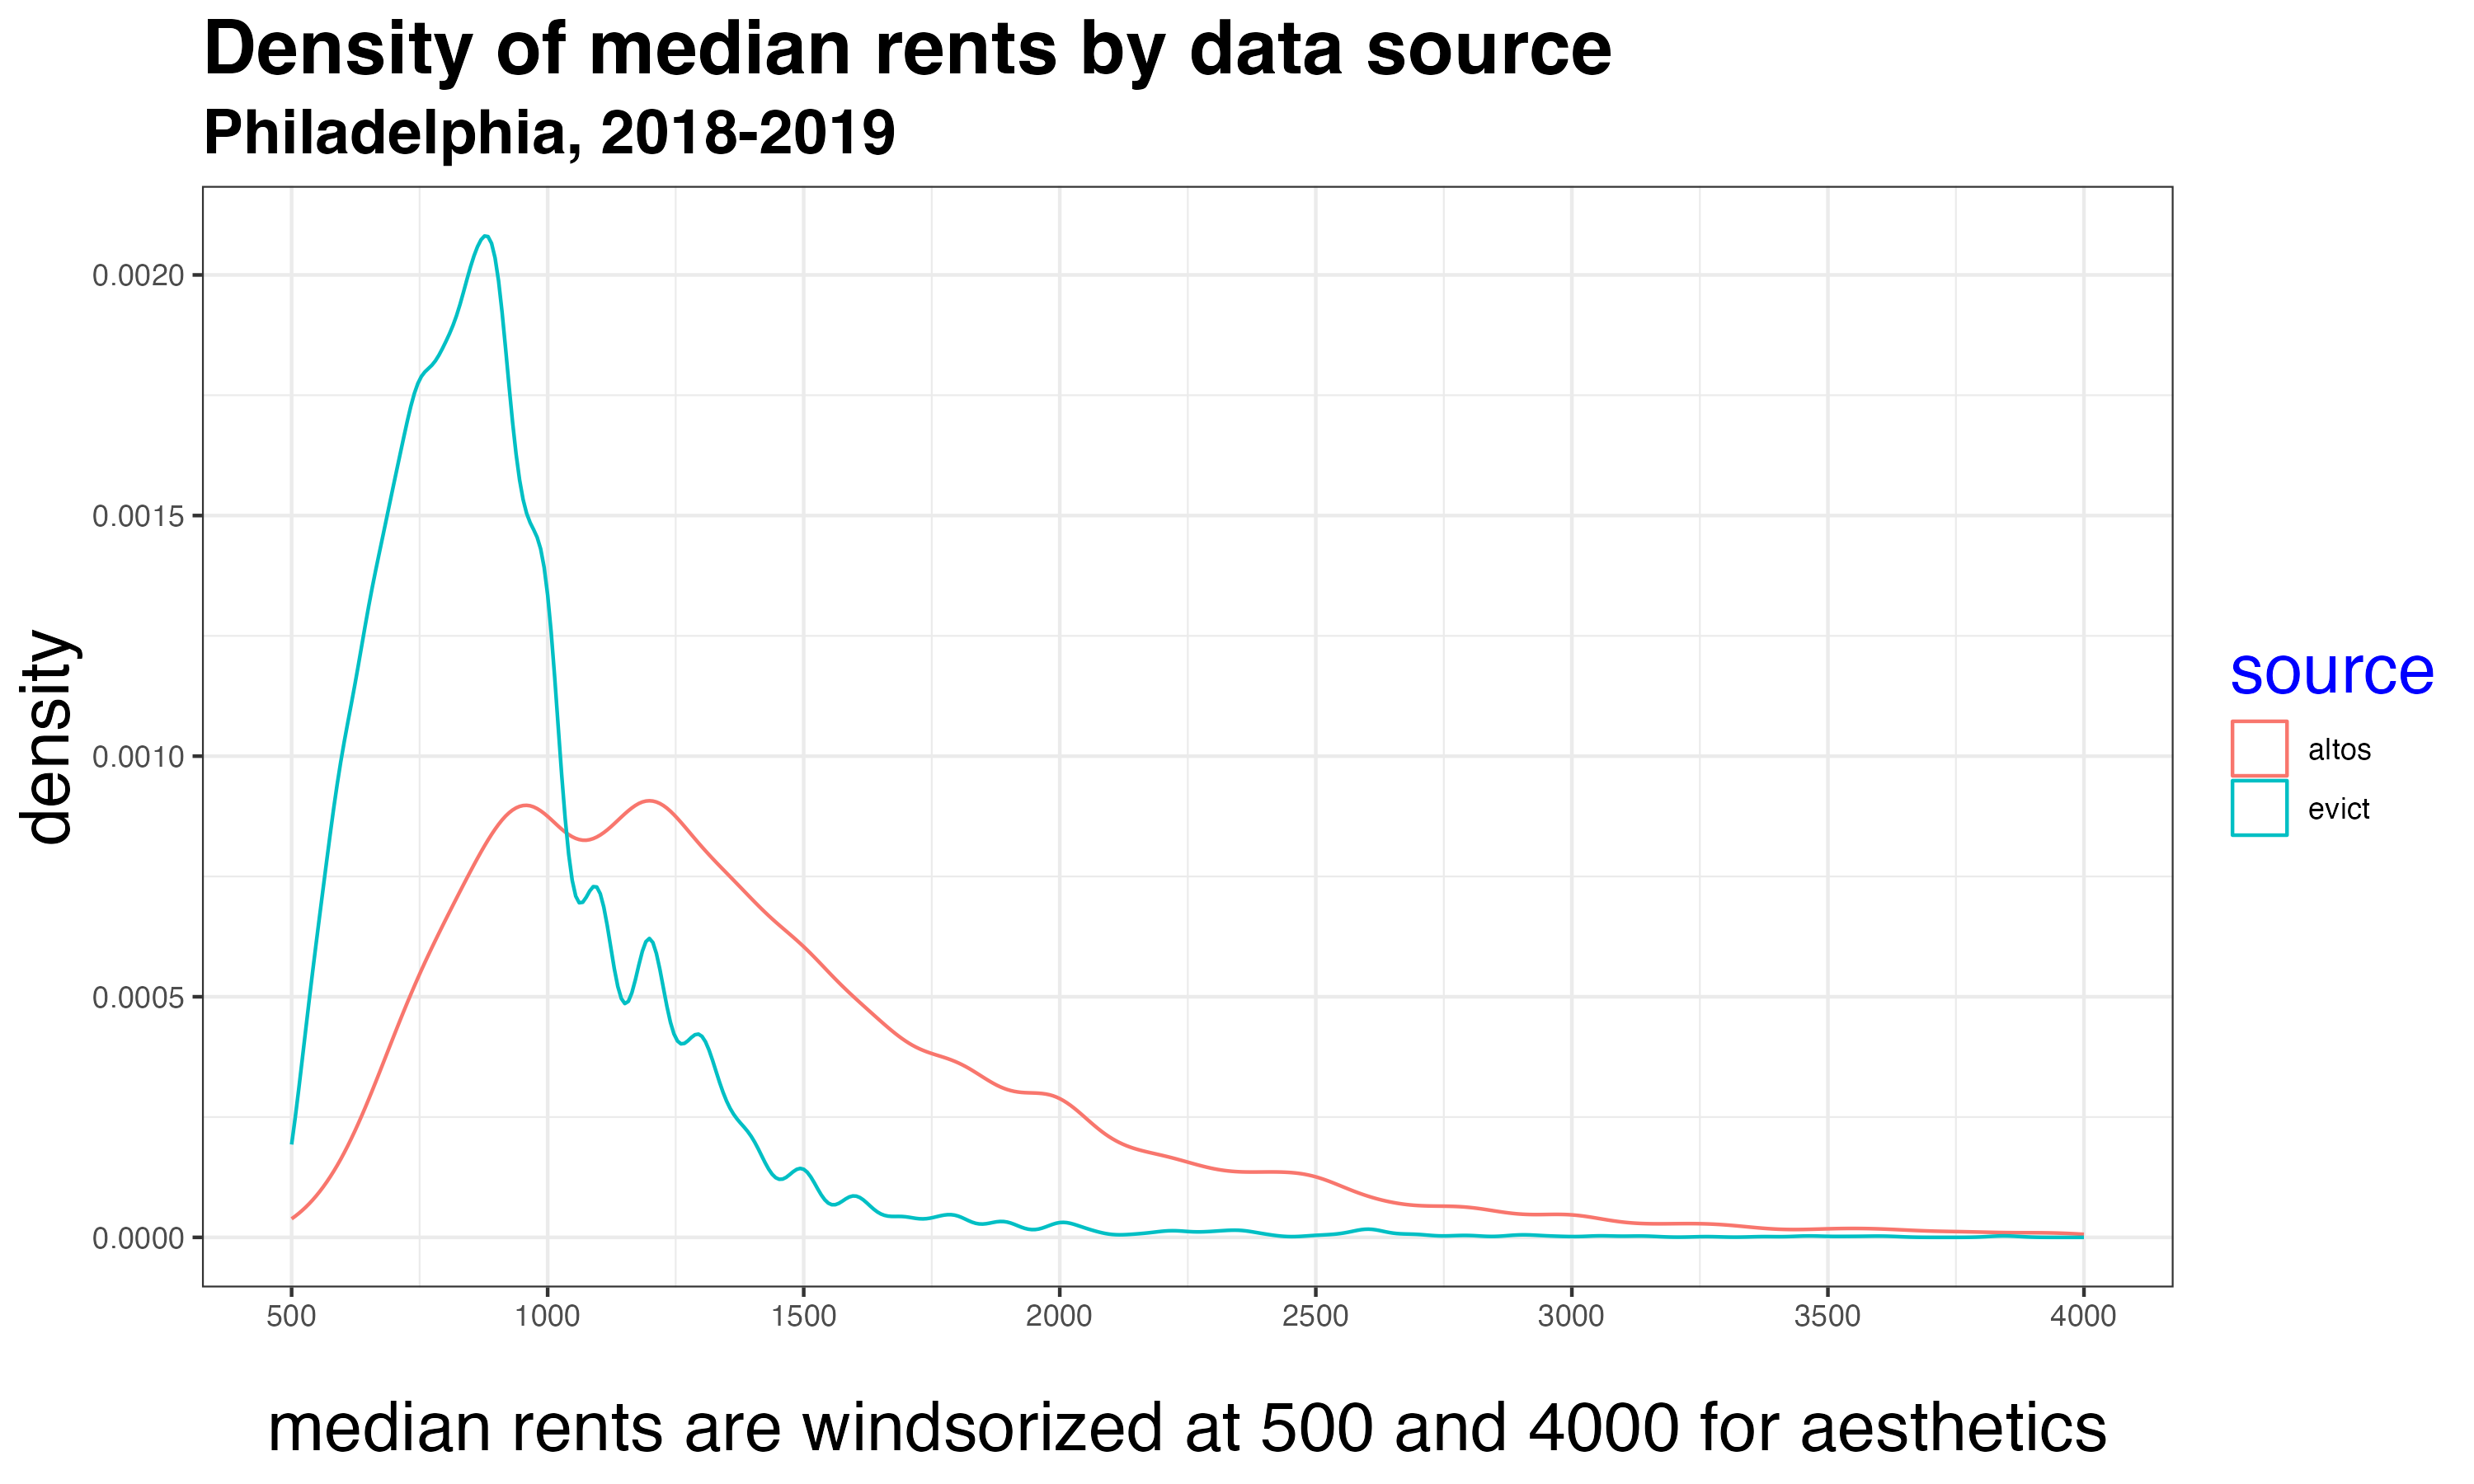
\includegraphics[width=1\linewidth]{figs/density_rent_prices.png}
        \caption{Rent Prices by Data Source}
        \label{fig:rent-dist}
    \end{figure}

Finally, on the policy side, Philadelphia had a large change in their tenant protections in 2022, where they now make eviction cases go through mediation, leading to an approximately 30\% decline in eviction filings, relative to a pre-pandemic baseline.

\clearpage

\section{Stylized Facts about Philadelphia's Low Income Housing Market}

\subsection{Hedonic Regressions}
In this section, I lay out a series of motivating empirical facts about Philadelphia's low income housing market. Begining with hedonic regressions, I document two facts about prices in high evicting units:

\begin{itemize}
    \item Unconditionally, eviction rates don't correlate with prices after a ~20\% filing rate
        \item After controlling for property and neighborhood characteristics, units with \textbf{higher} eviction rates charge \textbf{higher} rents 
\end{itemize}

In figure \ref{fig:bin-scatter}, I plot the bin scatter for inflation adjusted rent prices as a function of the property level filing rates.\footnote{The filing rate is the historical average number of filings per unit per year. So a building with 100 units that files 20 evictions in a typical year would have a filing rate of 0.2} I find that there is a steep negative relationship between filing rates and prices, however, this relationship turns flat after around 0.2, indicating that prices for a building that evicts 20\% of their tenants are comparable to a building that evicts 80\%.

\begin{figure}[htbp]
        \centering
        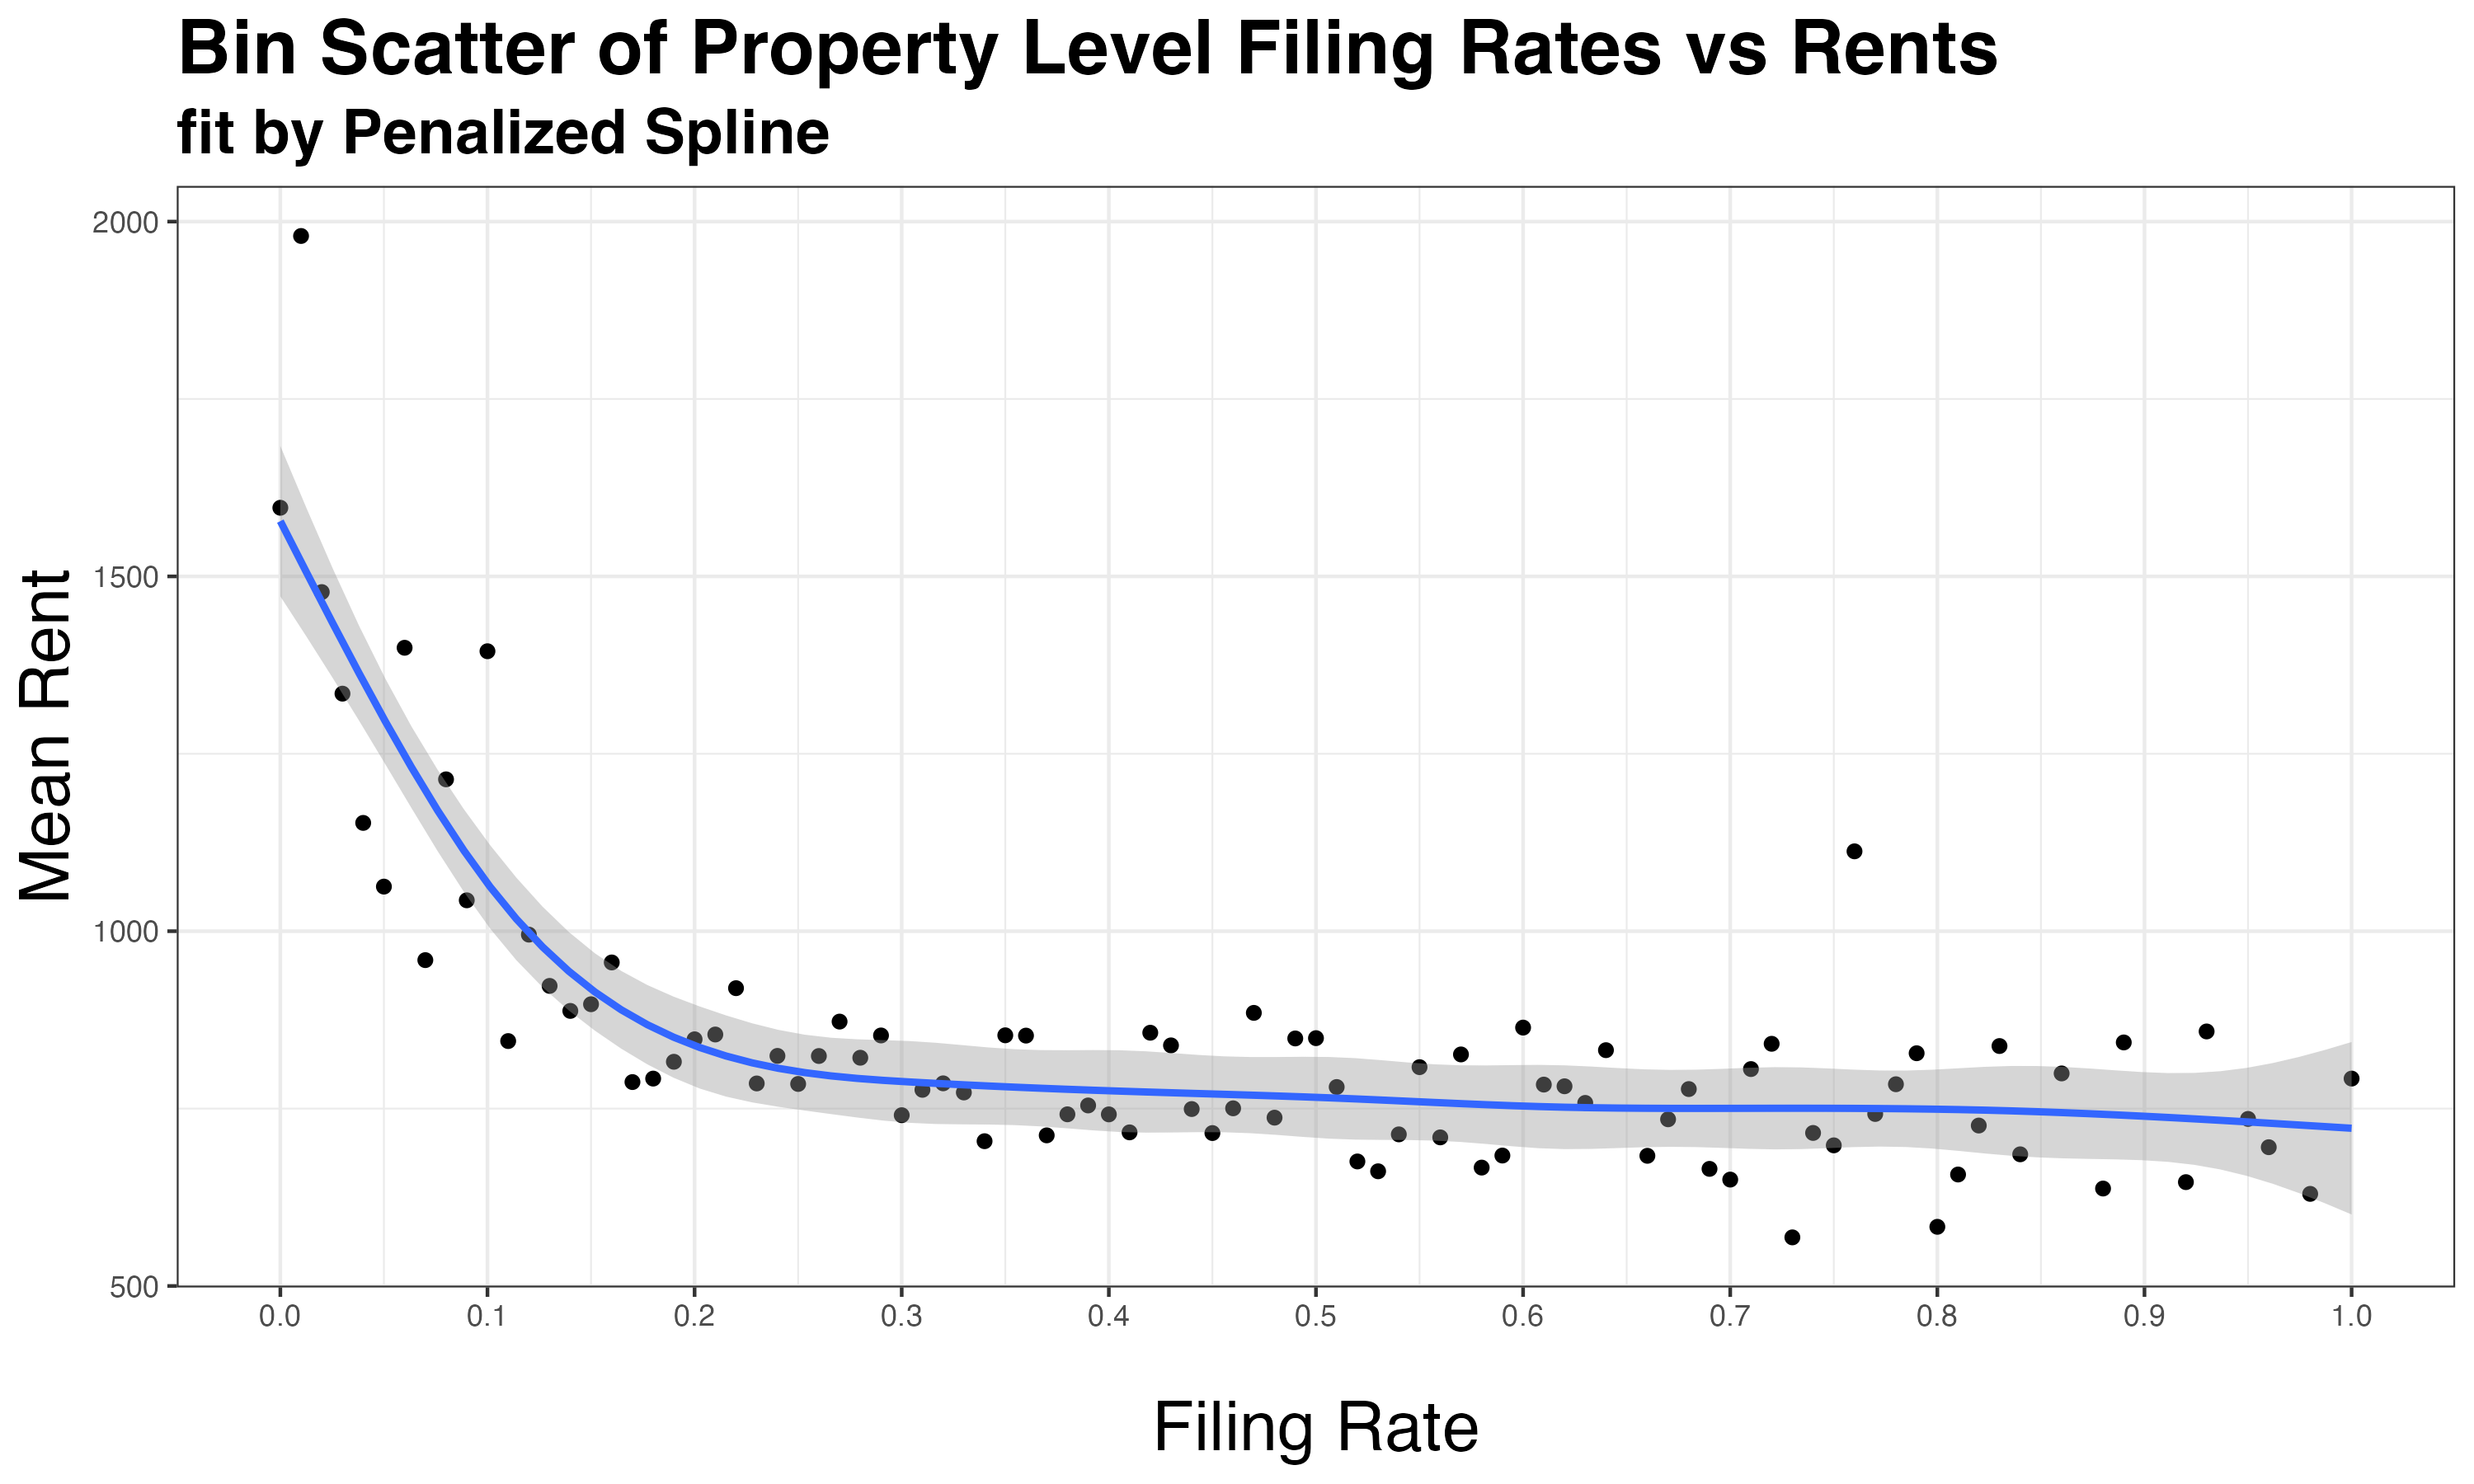
\includegraphics[width=1\linewidth]{figs/philadelphia_filing_rate_rent_scatter.png}
        \caption{Bin Scatter of Eviction Rates by Data Source}
        \label{fig:bin-scatter}
    \end{figure}

Next, in table \ref{tab:rent_regs}, I plot the results from a hedonic regression of prices on observables. In this regression, I subset the data to be only units that had an eviction filing. In the first column, I document that, unconditionally, there is a strong negative relationship between prices and filing rates. However, in column 2, after controlling for a large number of neighborhood and property characteristics, the coefficient on filing rates turns positive.

\begin{center}
        \begin{table}[htbp]
   \caption{\label{tab:rent_regs} Rent Price Regressions}
   \centering
   \begin{tabular}{lcc}
      \tabularnewline \midrule \midrule
      Dependent Variable: & \multicolumn{2}{c}{Log(Price)}\\
      Model:                       & (1)             & (2)\\  
      \midrule
      \emph{Variables}\\
      Filing Rate                  & -0.9082$^{***}$ & 0.0122$^{**}$\\   
                                   & (0.0888)        & (0.0054)\\   
      Polynomial Imputed Beds      & No              & Yes\\  
      Polynomial Imputed Baths     & No              & Yes\\  
      Polynomial Year Built        & No              & Yes\\  
      Polynomial Number of Stories & No              & Yes\\  
      Polynomial Number of Units   & No              & Yes\\  
      \midrule
      \emph{Fixed-effects}\\
      Year                         & Yes             & \\  
      Census Block Group-Year      &                 & Yes\\  
      Heater Type                  &                 & Yes\\  
      Quality Grade                &                 & Yes\\  
      View Type                    &                 & Yes\\  
      Building Code                &                 & Yes\\  
      Construction Type            &                 & Yes\\  
      \midrule
      \emph{Fit statistics}\\
      Observations                 & 55,848          & 54,315\\  
      R$^2$                        & 0.25091         & 0.84653\\  
      \midrule \midrule
      \multicolumn{3}{l}{\emph{Clustered (Parcel ID) standard-errors in parentheses}}\\
      \multicolumn{3}{l}{\emph{Signif. Codes: ***: 0.01, **: 0.05, *: 0.1}}\\
   \end{tabular}
\end{table}

\end{center}

Both of these facts are surpising as, intuitively, higher filing rates should correlate negatively with prices as higher filing rates are likely correlated with bad unobserved quality and households likely dislike high filing rates in and of themselves. These hedononics can't rule out high prices for high evicting units as representing default premia, however, previous literature on higher profits for low income rentals suggests default premia cannot explain everything.

\clearpage

\subsection{Market Segmentation}

In this section, I present some preliminary evidence on market segmentation. In the future, I will do this with the InfoUSA data to empirically document what kinds of properties low income renters are substituting between. In the absence of these data, I segment markets based on zip code and property type, following \parencite{framoutar2024market, calderwang2024algorithmic} and by whether the unit had an above 15\% average filing rate.  I'll show that, if you think because of tenant screening, low income renters substitute largely between high evicting properties, markets can be fairly consolidated.

\begin{figure}[htbp]
        \centering
        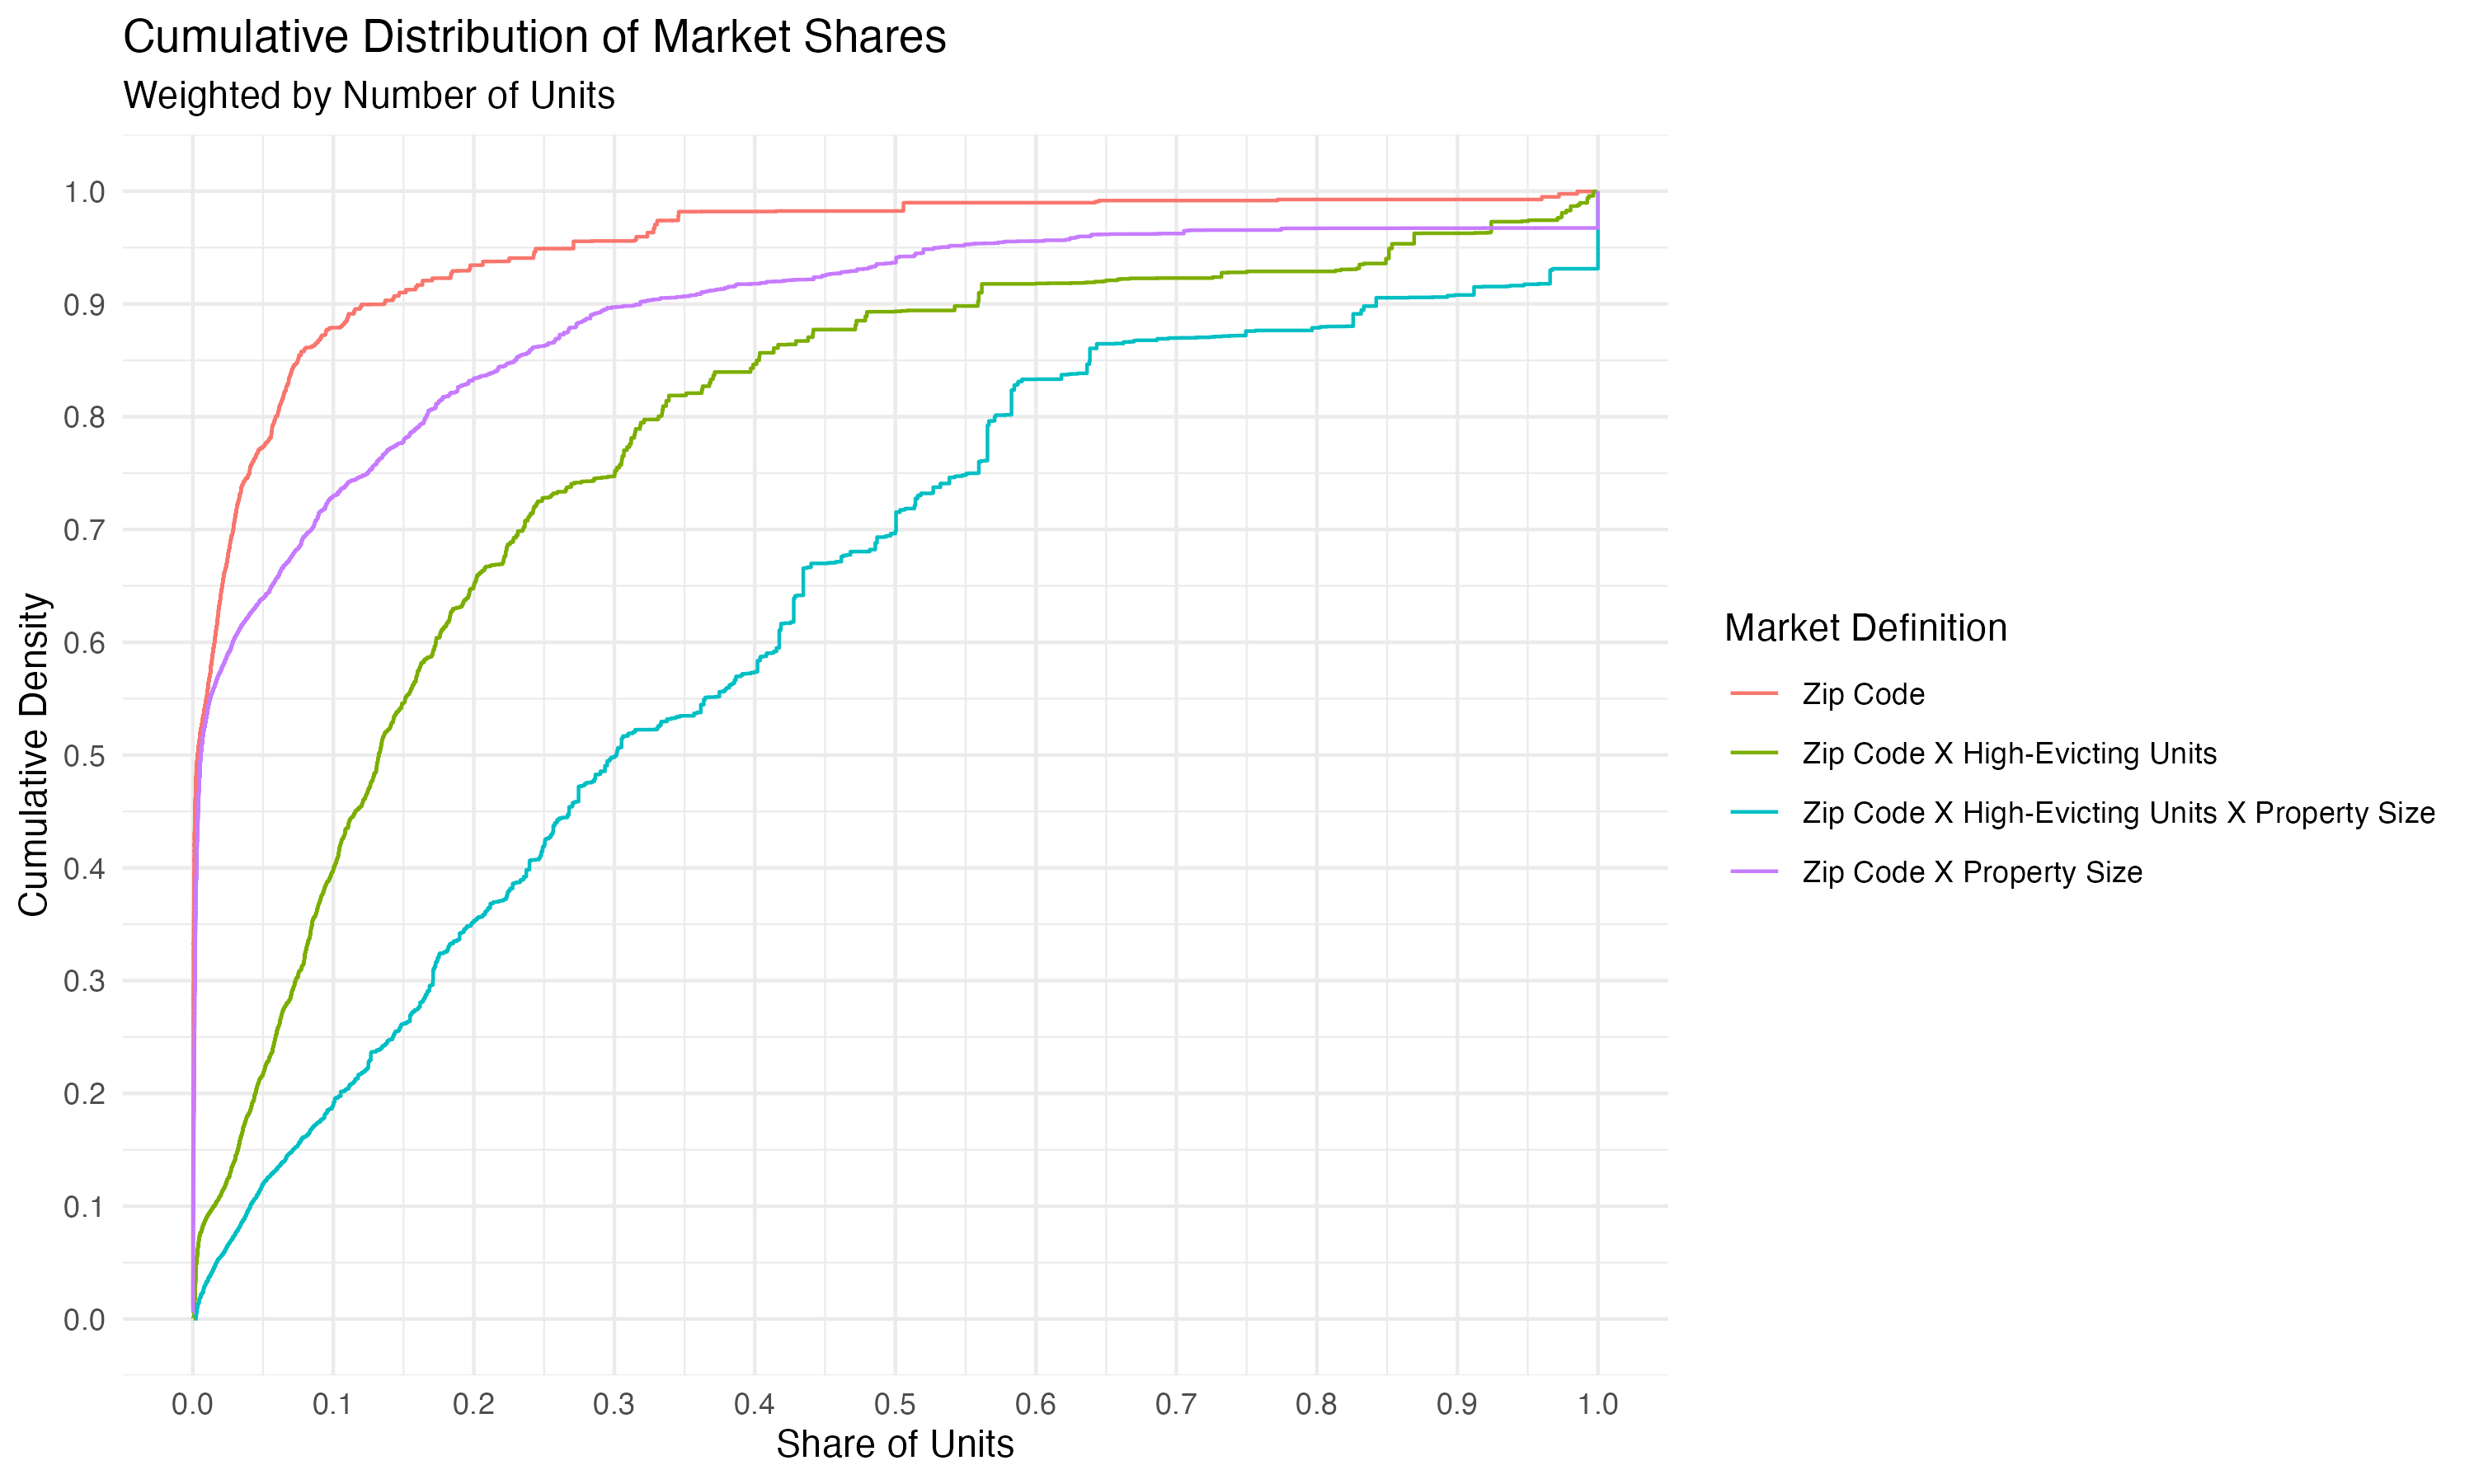
\includegraphics[width=1\linewidth]{figs/market_share_cdf.png}
        %\caption{Caption}
        \label{fig:market-share-cdf}
    \end{figure}

In figure \ref{fig:market-share-cdf}, I plot the CDF of market shares, that is, the percent of tenants who rent from a landlord who owns X\% or more of the market they rent in. Begining with the zip code and zip code by property type market definitions, I show that the overall rental market is not consolidated. However, if tenants are choosing between units that have at least a 15\% average filing rate within a zip code, around 20\% of tenants will rent from a landlord who owns at least 20\% of the units in their market. 

\subsection{Recap}
Taken together, I think there's evidence that prices in low income markets are "surpisingly" high and there's sufficient market consolidation that we might be worried about market power. In the next section, I turn to how I want to think about market power in this setting, which is that landlords internalize that their tenants have high search costs and poor outside options, and use that to raise rents.
% Beginning with a map of Philadelphia (figure \ref{fig:philly-map}), I show that evictions in Philadelphia are geographically very concentrated in the predominately poor and highly segregated neighborhoods of West and North Philadelphia.
\clearpage
\documentclass{article}
\usepackage{graphicx} % Required for inserting images
\usepackage{hyperref}
\usepackage{amsmath}
\usepackage{longtable}
\usepackage{booktabs}
\title{PAT paper}
\author{Joseph Fish}
\date{March 2024}


\begin{document}

\section{Motivation}

\textbf{Big Picture}: the Rental market behaves much more like the labor market than it does the car market. Firms post vacancies, tenants apply, contracts are bargained over, and posted units may or may not actually be available to tenants. This matters for how we think about market power and modelling the housing market. \\

\textbf{Why this matters}: Recent models of market power in housing market model the supply side with differentiated Bertrand competition (sometimes Cournot), where market power comes from product differentiation and quantity reduction. The first issue is that implied elasticities from empirical estimates of prices and vacancies are not consistent with elasticities from demand estimation. The second issue is that, because most housing was built decades ago, firms can only move around quantities by:\\
\begin{enumerate}
    \item internalizing market power at time of development (unlikely for old buildings)
    \item moving around quantities by changing vacancy rates, in which case search is the natural way to think about the problem
\end{enumerate}


In particular, it's  likely that landlords flex monopoly power by exploiting search costs and influencing tenants' outside options. One simple example of this is that they can exploit tenant switching costs

\section{Intuition}
To fix intuition, consider two markets of 1000 units each. In market 1, there are 100 landlords who each lease 10 units. In market 2, there are 10 landlords leasing 100 units each. Standard competition models say that as long as their vacancy rates are the same, so will market prices. I think this is weird!

\section{Empirical Example}

Take this job market paper from this year. The first figure is the results from a Diff in Diff on mergers of rental properties, filtered for mergers that increase concentration by a substantial amount. She estimates prices effects in the order of 7.5\%. \footnote{You can square this result with my field paper that shows no effect of these kinds of mergers by noting that she filters for mergers that are in the top 5\% of changes in predicted concentration; likely the total ATT is zero} She then explains this by noting that firms also increase vacancies concurrently with hiking prices (and that it doesn't look like they're doing unobserved quality upgrading). However, she finds vacancy effects in the order of a 5\% decline in \textit{own supply}. This would imply own price elasticities of around -0.66. If the coefficients on vacancies are percents (one, this is implausible, as occupancy rates do not hit low 70s), you get an elasticity of -2.66, which is technically plausible, but inconsistent with her estimates of demand elasticities later in the paper. 


\section{RealPage}
RealPage is an example of where I think firms actually are doing Bertrand style quantity reduction. However, I think this makes my point: with RealPage, market vacancy rates get reduced by ~3\% and prices go up by 3-5\%. This is a much more normal effect than what other people are finding.


\section{Model}

\subsection{Setup}

\begin{itemize}
    \item Discrete time economy
    \item unit measure of infinitely lived, homogenous renters
    \item renters are either housed and pay rent ($r$) to receive flow utility or are unhoused
    \item Common discount factor $0 < \beta < 1$
    \item housed renters experience exogenous separation shock at rate $\delta$
\end{itemize}

\subsection{Matching}
\begin{itemize}
    \item For each rental vacancy, firms pay a per period cost of $c_i$
    \item Urn-ball matching function. Each period, $u$ unemployed workers send one application (balls) towards $v$ vacancies (urns).
    \begin{itemize}
        \item Due to coordination frictions, some vacancies see $>1$ applications and some see zero. Applications per vacancy are exponentially distributed
    \end{itemize}
    \item If a firm gets multiple applicants, they select one at random to follow up with and bargain over rents
    \begin{itemize}
        \item Nash bargaining; $0 \leq \alpha \leq 1$
        \item In this model, firms aren't allowed to have applicants bid up the rents (unclear why this couldn't be allowed, but I don't do it here)
        
    \end{itemize}
    \item Tenants are assumed to search randomly within a market (equivalent to vacancies appearing randomly); no directed search. This will be important later.
    \item Home finding rate = $\lambda \equiv \frac{v}{u}(1-e^{-\frac{v}{u}})$
\end{itemize}

\subsection{Worker Value Functions}
\begin{itemize}
    \item U = value of outside option (homelessness; living in non-preferred neighborhood); R = rent paid
    \item \begin{equation}
        U = b + \left(\lambda \sum_{i} f_iW_i + (1-\lambda)U\right)\label{eq:worker-val}
    \end{equation}
\end{itemize}

\subsection{Threat and Market Power}
\begin{itemize}
    \item In eq \ref{eq:worker-val}, firms compete with themselves because the firm's other vacancies enter the worker's outside option
    \item What firms can do instead is (partially) remove themselves from the tenants' outside option by committing themselves to not renting to the tenant in the future in the event bargaining breaks down.
    \begin{itemize}
        \item This commitment works by firm's choosing applicants randomly but removing the tenant in the event they have multiple applicants.
        \item Importantly, this is costless to the firm, since they have multiple applicants. (If the deviating tenant is sole applicant, they get the unit)
    \end{itemize}
    \item Here, I say that this punishment lasts until the tenant's search is over, so landlords need only be able to recognize a tenant's application for a short period of time
    \begin{itemize}
        \item Intuitively, one could imagine a property manager making an take it or leave it offer to a tenant with the threat that if they leave it they can't see other units
    \end{itemize}
    \item Continuation value in event of breakdown:
    \begin{equation}\label{eq:match-val}
        U_i = b + \beta \left(\lambda\sum_{j\neq}f_iW_j + \lambda f_iW_i + (1-\lambda(1-f_i) - \lambda f_i)U_i\right)
    \end{equation}
\end{itemize}

\subsection{Firm Value Function}
\begin{itemize}
    \item Bilateral value of match \begin{equation}
        J_i = 1 - w_i + \beta(1 - \delta)J_i
    \end{equation} 
    \begin{itemize}
        \item Value of landlord i of filling vacancy is flow output minus wage (maybe change to rent minus costs?)
    \end{itemize}
    \item \begin{equation}\label{eq:job-value}
        V_i = -c_i + \beta(1  - e^{-\frac{u}{v}})J_i
    \end{equation}
    \begin{itemize}
        \item Value of vacancy is fixed cost plus probability firm has at least one application; in equilibrium trade never breaks down and the match is always formed (how to think about tenant screening?)
    \end{itemize}
    \item \begin{equation}\label{eq:surplus-value}
        S_i \equiv W_i = U_i + J_i
    \end{equation}
    \begin{itemize}
        \item Joint value of surplus is then 
    \end{itemize}
    \item Assume nash bargaining:
    \begin{itemize}
        \item Worker Split: \begin{equation}\label{eq:nash-worker}
            aS_i = W_i - U_i
        \end{equation}
        \item Firm Split: \begin{equation}
            (1-\alpha)S_i = J_i
        \end{equation}
    \end{itemize}
\end{itemize}

\subsection{Closing the Model}
\begin{itemize}
    \item Assume free entry
    \begin{itemize}
        \item Is this correct for housing?
        \item Is this necessary? Can just close by saying no entry? Some landlords are just lucky?
    \end{itemize}
\end{itemize}

\subsection{Concentration Index}

\section{}{Data (Lol)}

\subsection{Market Definition}

\subsection{Needed Variables}

\end{document}

% \begin{figure}[htbp]
%     \centering
%     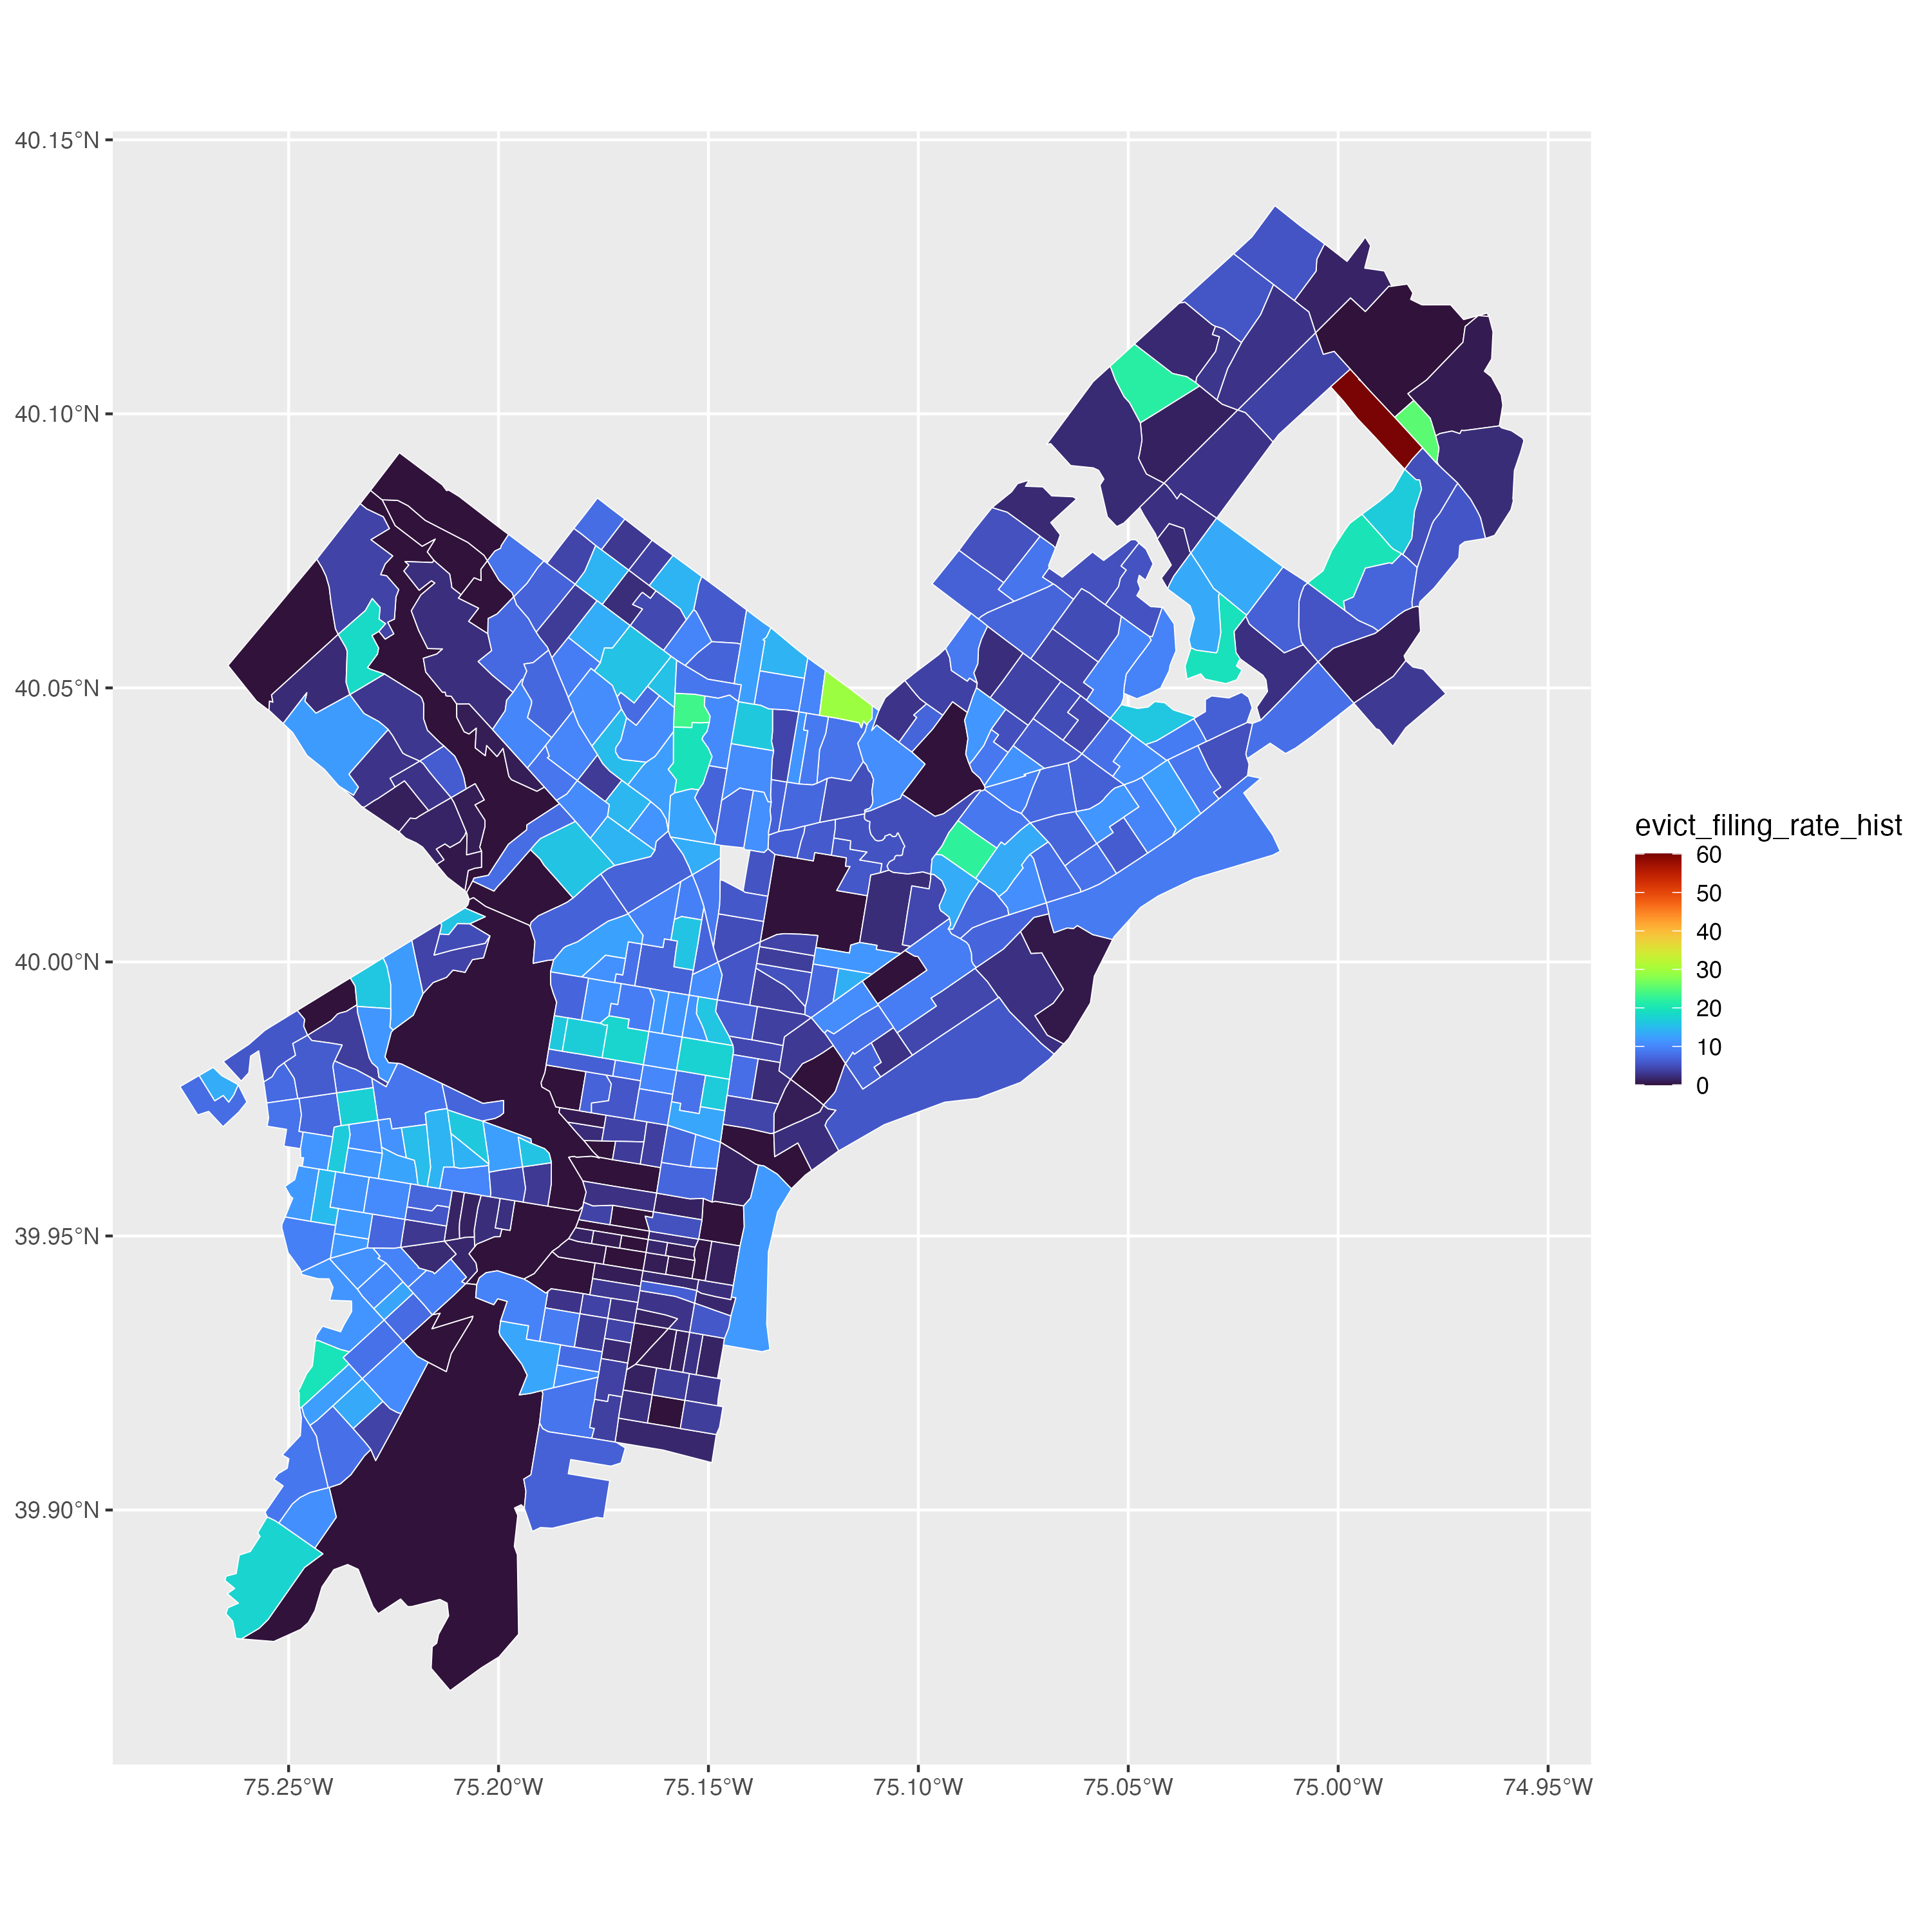
\includegraphics[width=1\linewidth]{figs/evict_filing_rate_hist.png}
%     \caption{Evictions in Philadelphia (2019)}
%     \label{fig:philly-map}
% \end{figure}

% Secondly, I show that, when looking across properties, evictions are concentrated in a handful of buildings. To show this, I merged the eviction data, which contain the defendant's address, with the rental registry and the parcel data in Philadelphia. This lets me know which properties are rental units in a given year, as well as the number of rental units that are in each property. Doing this allows me to plot the CDF of eviction filings alongside the CDF of rental units. \\

% As figure \ref{fig:philly-evict-parcel} shows, the vast majority of rental units do not file an eviction in a typical year. Of the properties that do file an eviction, most file only one. Collectively, about 10\% of all eviction filings come from just 2\% of units. \\

% \begin{figure}[htbp]
%     \centering
%     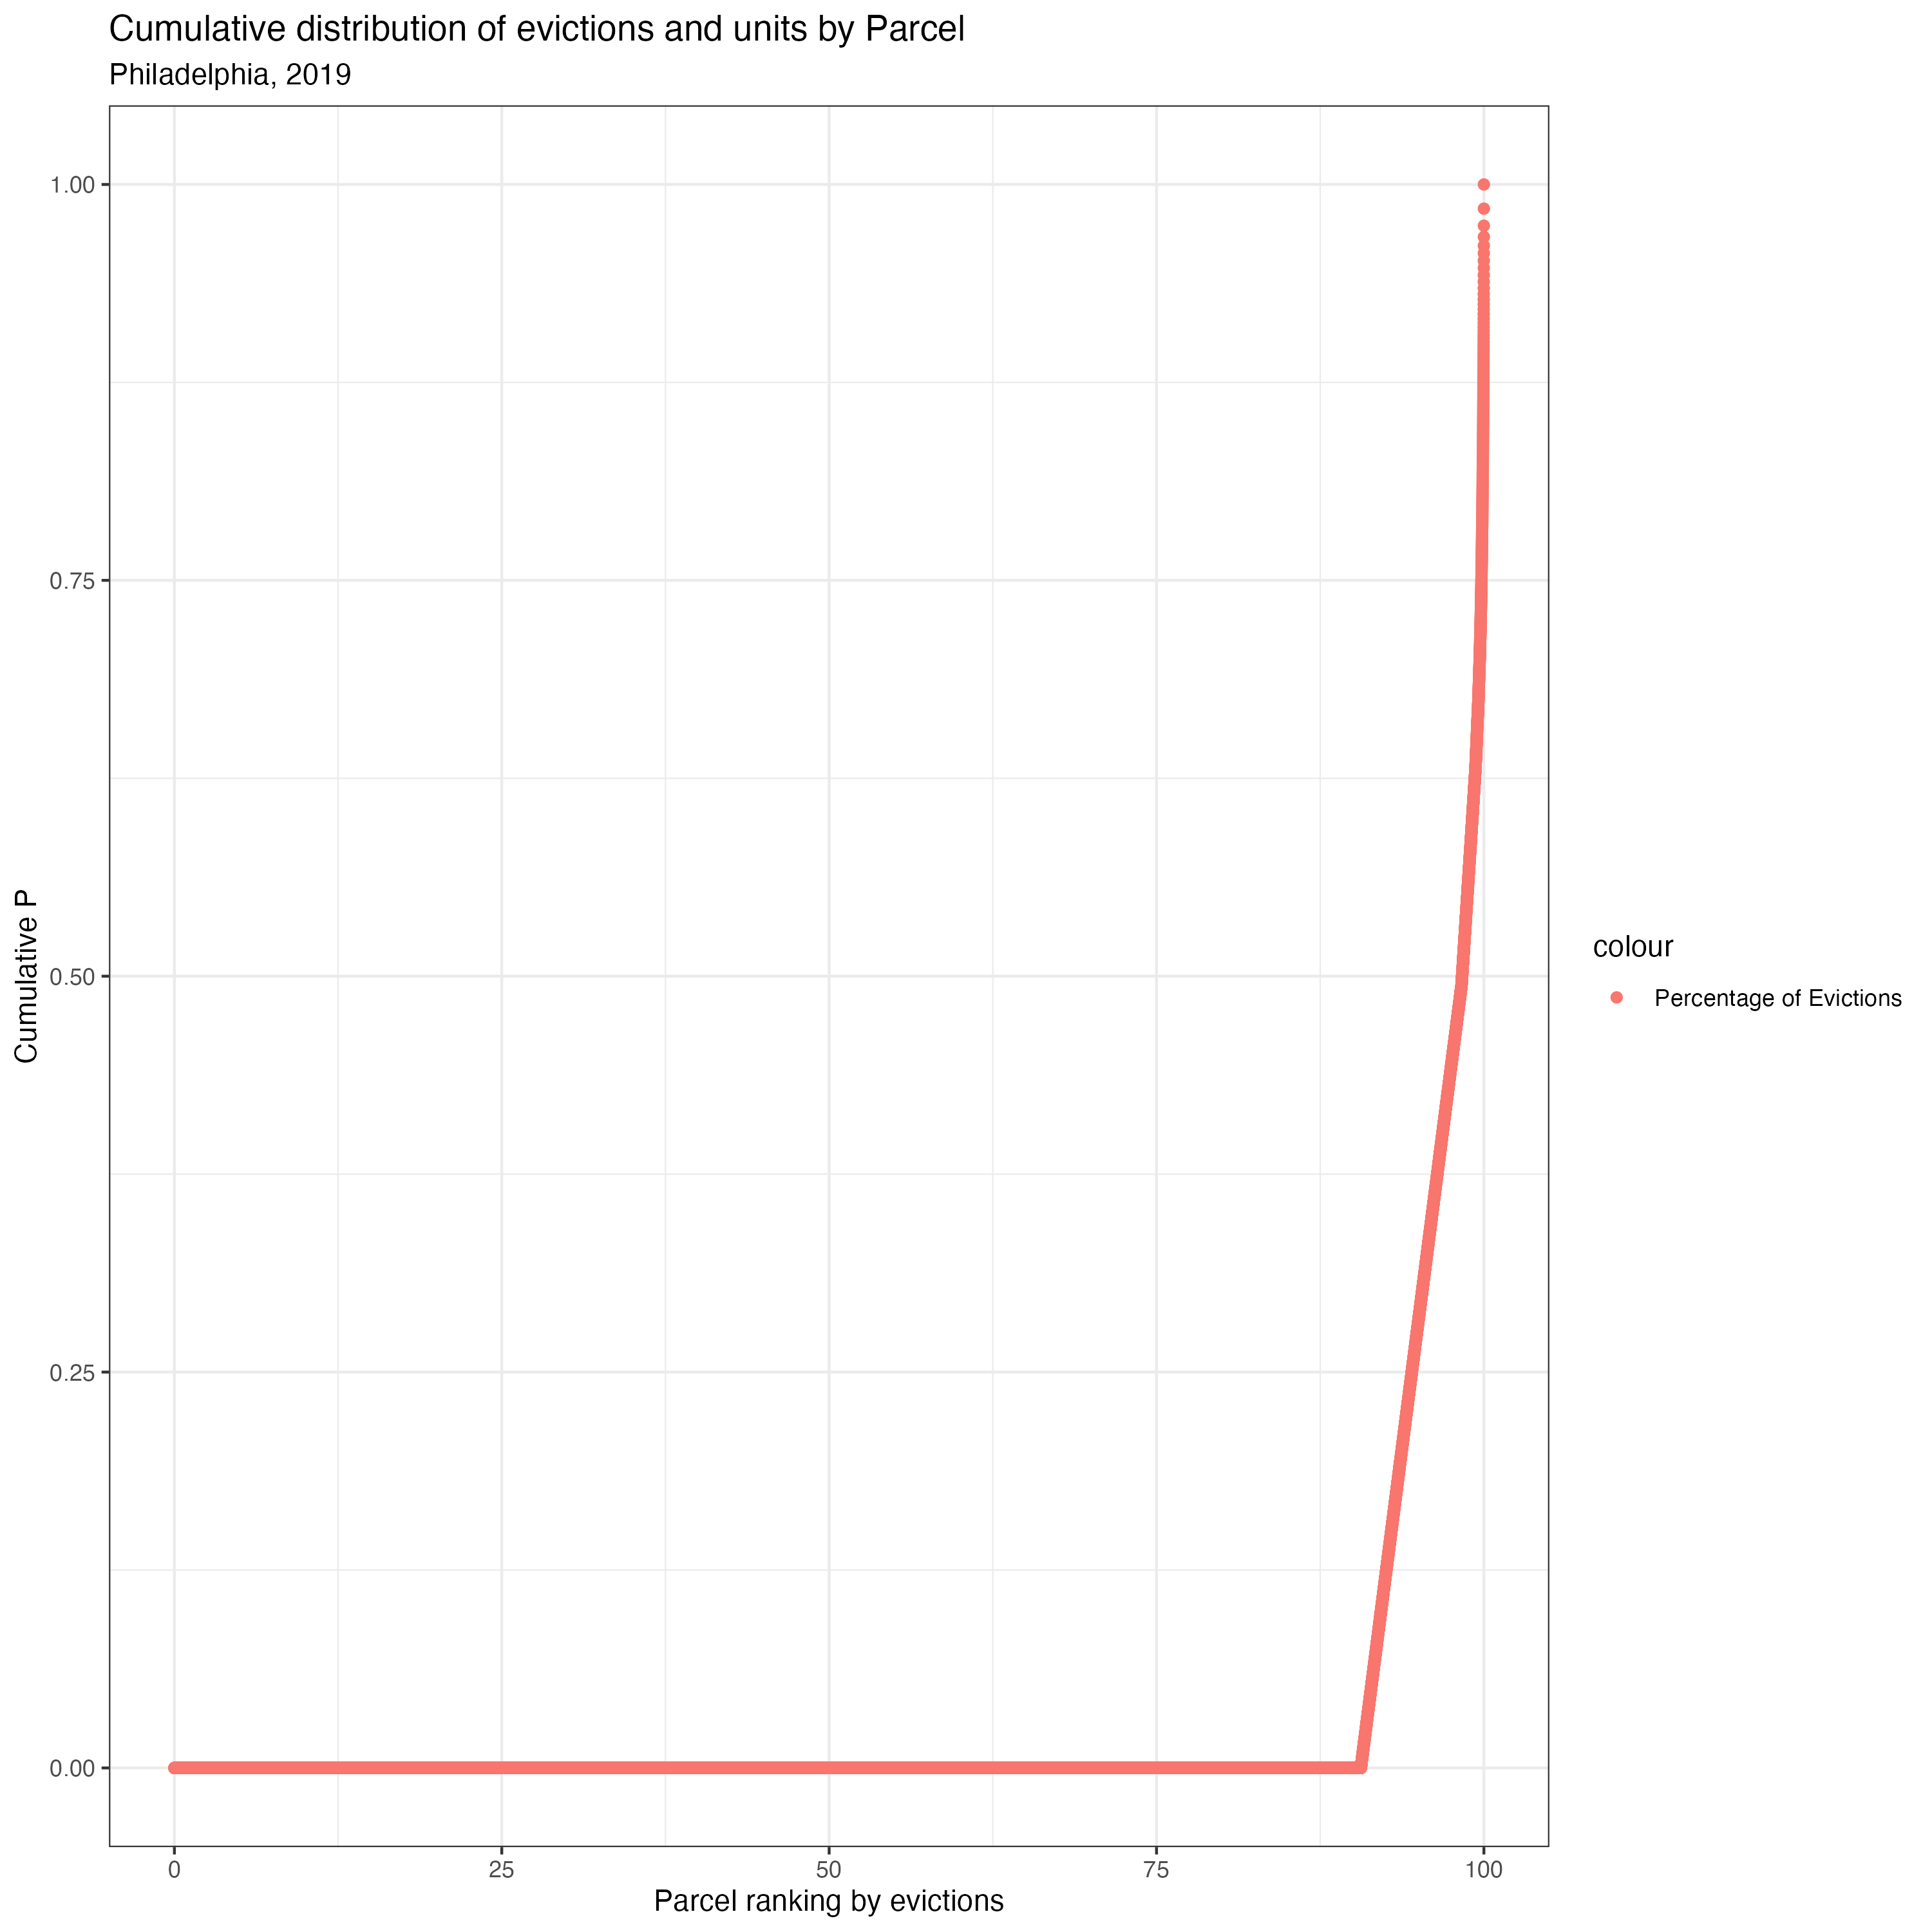
\includegraphics[width=1\linewidth]{figs/cumulative_evict_dist_parcels.png}
%     \caption{Evictions in Philadelphia}
%     \label{fig:philly-evict-parcel}
% \end{figure}

% Third, in table \ref{tab:philly-rent},I group eviction filings by whether they were filed by one of the top-100 evicting plaintiffs in each year. I show that there are not substantial differences in rent prices between filings by high / low evicting plaintiffs.\\

% \begin{table}[htbp]
%     \begin{longtable}{l|rrrr}
\caption*{
{\large Summary Statistics on Philadelphia Rent Prices} \\ 
{\small 2010-2019}
} \\ 
\toprule
\multicolumn{1}{l}{} & \multicolumn{2}{c}{Rent} & \multicolumn{2}{c}{Number of Evictions} \\ 
\cmidrule(lr){2-3} \cmidrule(lr){4-5}
\multicolumn{1}{l}{} & non-Top Evictor & Top Evictor & non-Top Evictor & Top Evictor \\ 
\midrule\addlinespace[2.5pt]
2010 & $675$ & $634$ & 14649 & 6674 \\ 
2011 & $685$ & $654$ & 14979 & 6498 \\ 
2012 & $700$ & $654$ & 15271 & 6642 \\ 
2013 & $700$ & $675$ & 15366 & 6064 \\ 
2014 & $725$ & $707$ & 15645 & 6257 \\ 
2015 & $750$ & $725$ & 14395 & 5891 \\ 
2016 & $750$ & $800$ & 14994 & 5622 \\ 
2017 & $775$ & $825$ & 14627 & 5748 \\ 
2018 & $800$ & $970$ & 11987 & 3735 \\ 
2019 & $850$ & $1,050$ & 11763 & 3473 \\ 
\bottomrule
\end{longtable}


%     \caption{Philadelphia Rent}
%     \label{tab:philly-rent}
% \end{table}


% Finally, in figure \ref{fig:philly-year}, I show that evictions declined substantially during COVID and have held at lower rates than the pre-pandemic baseline. \\

% \begin{figure}[htbp]
%     \centering
%     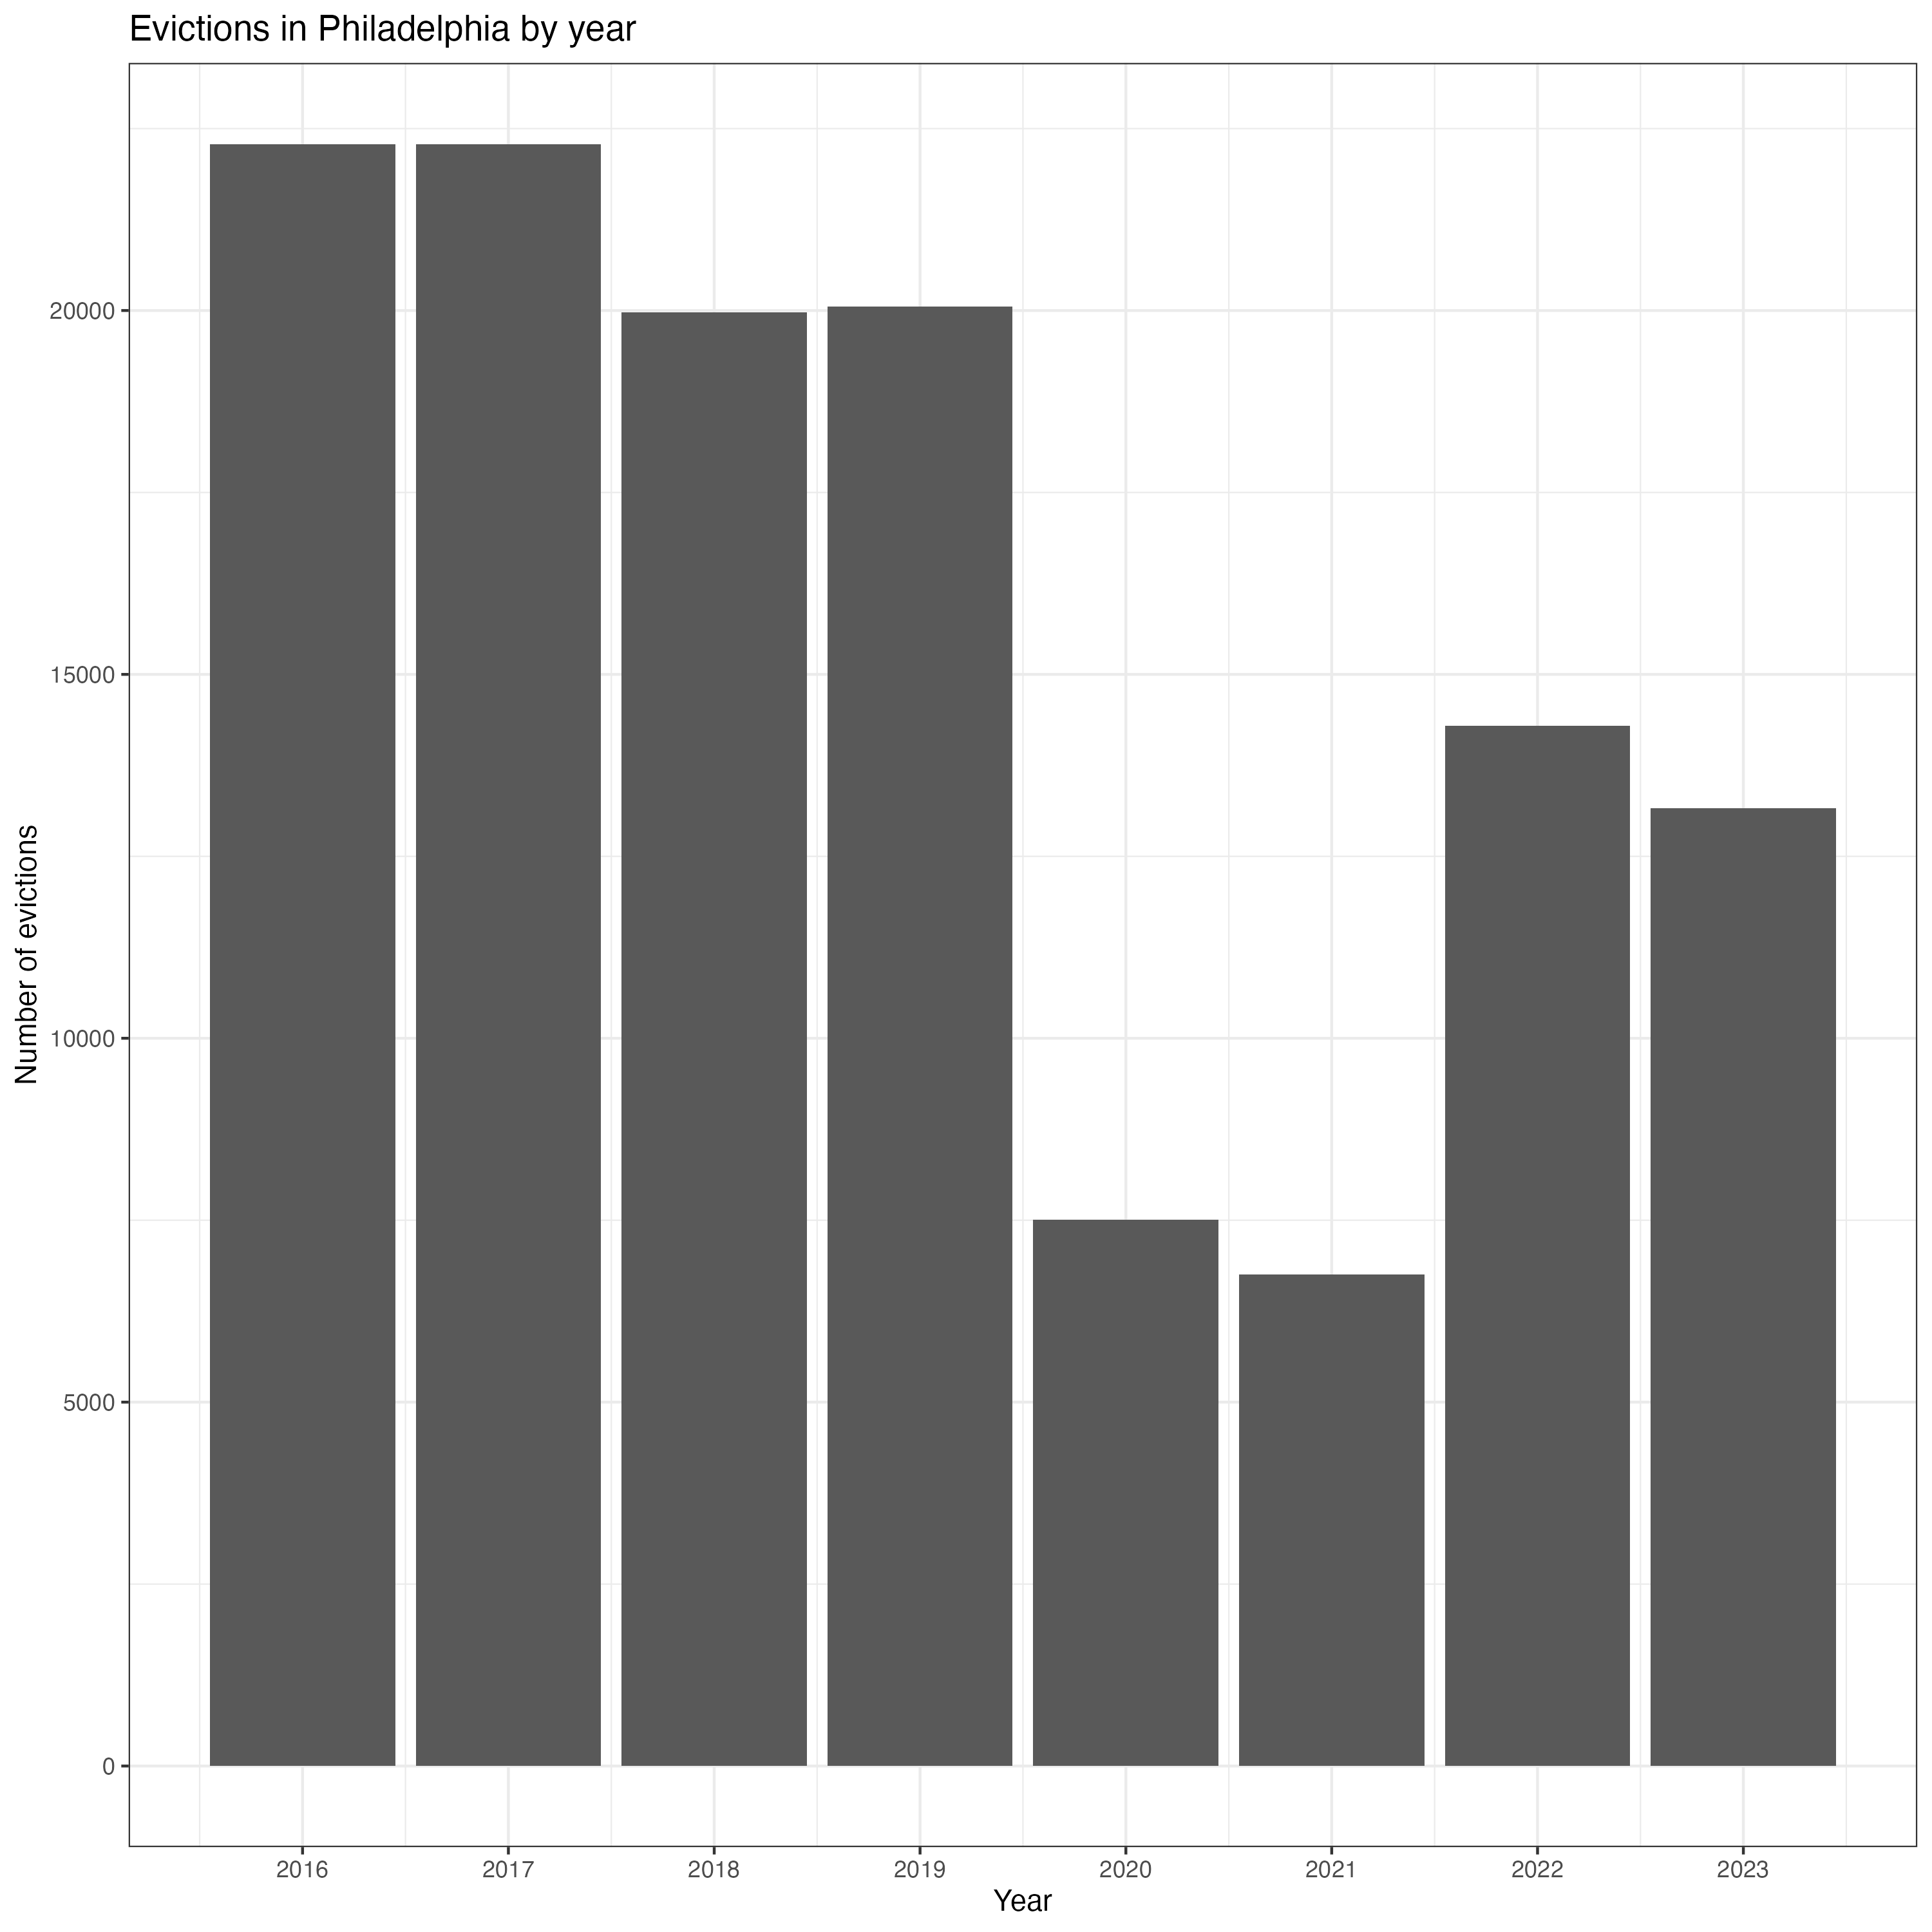
\includegraphics[width=1\linewidth]{figs/evict_by_year.png}
%     \caption{Evictions in Philadelphia}
%     \label{fig:philly-year}
% \end{figure}

% Taken together, these empirical facts show that there are interesting patterns of spatial clustering, patterns of landlord behavior, and possible policy variation I could exploit.
% \pagebreak
% \section{Research Questions and Empirical Specifications}

% \subsection{Descriptive Evidence on Pricing and Eviction Filing Behavior}

% The first set of findings I'd like to document are related to landlord pricing and filing behavior. Specifically:

% \begin{itemize}
%     \item Do high evicting landlords charge higher rents relative to similar properties?
%     \item Are thresholds (back rent required for eviction filing to occur) for high evicting landlords different from those for lower evicting landlords. 
%     \item Building on Alison Lodermeier's job market paper, a natural question would be whether high evicting landlords are more likely to statistically or tasted-basely discriminate against their tenants, relative to lower evicting landlords 
%     \item Are high evicting landlords also likely to be serial evictors -- meaning they use eviction both as a debt collection tool and as one to remove tenants.
% \end{itemize} \\

% As these are all descriptive findings, I think the identification is relatively straightforward. The main consideration will be what "similar property" means -- I think for now it will be defined geographically, assuming there aren't large rental gradients within the same neighborhood.



\end{document}